\documentclass[12pt, spanish]{ociamthesis}  % default square logo 
%\documentclass[12pt,beltcrest]{ociamthesis} % use old belt crest logo
%\documentclass[12pt,shieldcrest]{ociamthesis} % use older shield crest logo

%load any additional packages
\usepackage{amssymb}
\usepackage[spanish]{babel}
\usepackage[utf8]{inputenc}
\usepackage{url}

%input macros (i.e. write your own macros file called mymacros.tex 
%and uncomment the next line)
%\include{mymacros}

\title{Distribuciones de \\[1ex]     %your thesis title,
        probabilidad contínuas}   %note \\[1ex] is a line break in the title

\author{Alexander Baquiax}             %your name
\college{Universidad Galileo}  %your college

%\renewcommand{\submittedtext}{change the default text here if needed}
\degree{Estadística Matemática}     %the degree
\degreedate{Mayo 2017}         %the degree date

%end the preamble and start the document
\begin{document}

%this baselineskip gives sufficient line spacing for an examiner to easily
%markup the thesis with comments
\baselineskip=18pt plus1pt

%set the number of sectioning levels that get number and appear in the contents
\setcounter{secnumdepth}{3}
\setcounter{tocdepth}{3}


\maketitle                  % create a title page from the preamble info
\include{dedication}        % include a dedication.tex file
\include{abstract}          % include the abstract

\begin{romanpages}          % start roman page numbering
\tableofcontents            % generate and include a table of contents
%\listoffigures              % generate and include a list of figures
\end{romanpages}            % end roman page numbering

%now include the files of latex for each of the chapters etc
\chapter{Distribución T de Student}

Esta distribución surge de la necesidad de estimar la \textbf{media} de una población normalmente distribuida pequeña. \cite{wiki:1}

\section{Descripción}

Aparece de manera natural al realizar la prueba t de Student para la determinación de las diferencias entre dos medias muestrales y para la construcción del intervalo de confianza para la diferencia entre las medias de dos poblaciones cuando se desconoce la desviación típica de una población y ésta debe ser estimada a partir de los datos de una muestra.


\section{PDF}
\begin{center}
	$P(X=\textit{x}) = \frac{\Gamma((v + 1) / 2)} {\sqrt{v\pi} \Gamma (v/2)} (1 + x^2 / v)^{-(v+1)/2} $
\end{center}

\subsection{Parámetros}
Los parámetros que usamos en las funciones de esta distribución son:

\begin{center}
	\begin{tabular} {| l | l |}
		\hline
		v & Grados de libertad \textit{N} $\in 1, 2, 3, ...$\\ \hline
	\end{tabular}
\end{center}

\section{CDF}
La función de distribución acumualada es:

\begin{center}
$\frac{1}{2} + x\Gamma(\frac{v+1}{2}) \frac{H}{\sqrt{v\pi} \Gamma (v/2)}$
\end{center}

Donde \textit{H} es la función Hipergeométrica.

\section{Media y Varianza}
\subsection{Media}
La esperanza de una variable aleatoria X con distribución hipergeométrica es:
\begin{center}
	$0$
\end{center}

\subsection{Varianza}
siendo su varianza
\begin{center}
	$\frac{v}{v-2}$
\end{center}

\section{MGF}
\textit{No definida}

\section{Gráficas}

\begin{center}	
	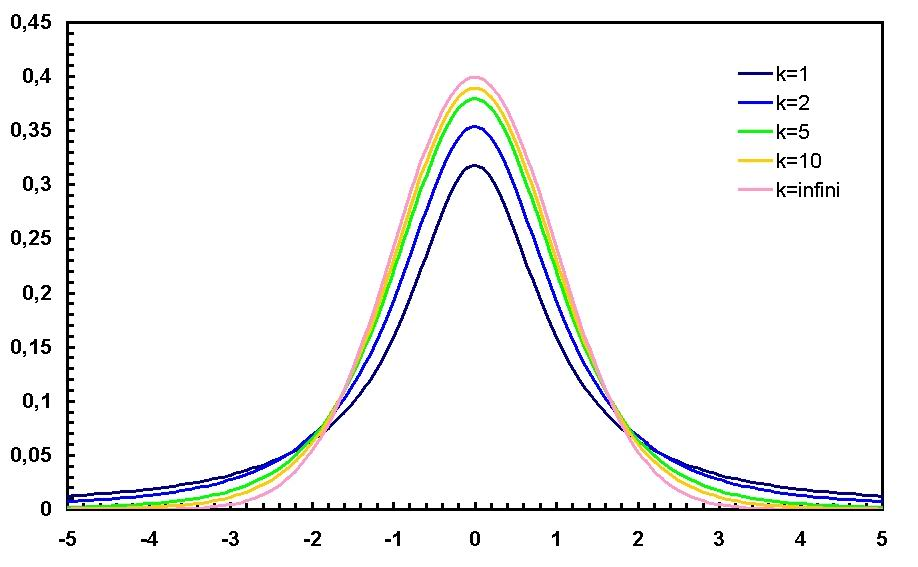
\includegraphics[scale=0.5]{imgs/t-pdf.jpeg}
	
	\textit{PDF}
\end{center}

\begin{center}	
	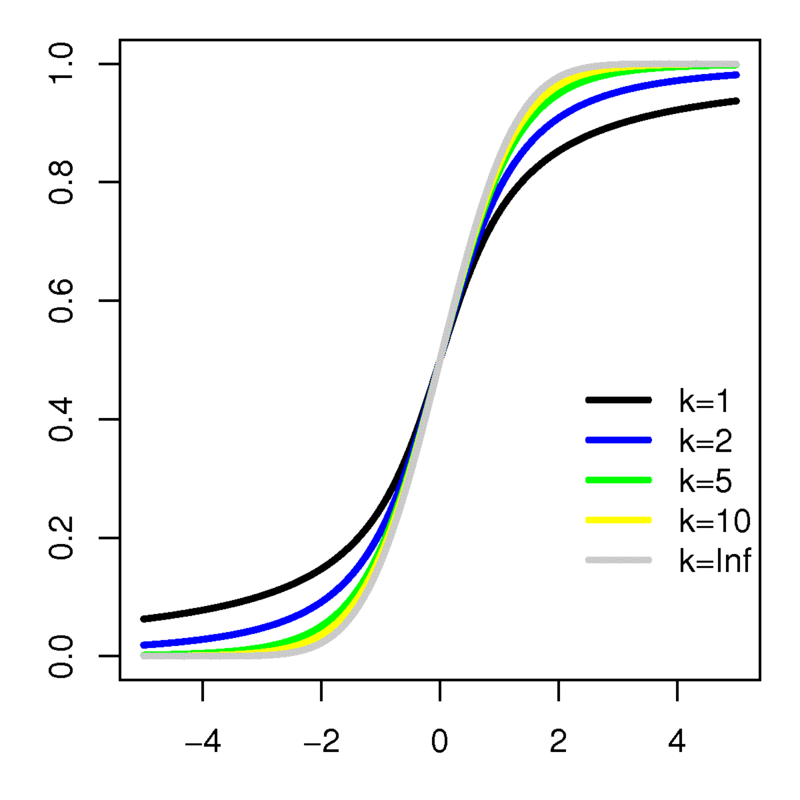
\includegraphics[scale=2]{imgs/t-cdf.png}
	
	\textit{CDF}
\end{center}


\section{Aplicaciones en la vida real}

Es aplicable cuando tenemos menos de 30 datos, y no conocemos la desviación estándar de la población y cuando la población de la extraemos la muestra está distribuida normalmente.
\chapter{Distribución F}
Usada en teoría de probabilidad y estadística, la distribución F es una distribución de probabilidad continua. También se le conoce como distribución F de Snedecor (por George Snedecor) o como distribución F de Fisher-Snedecor (por Ronald Fisher).


\section{Descripción}
La distribución F es una distribución continua de muestreo de dos variables aleatorias independientes con distribuciones de chi-cuadrado, cada una de las cuales se divide entre sus grados de libertad. \cite{wiki:2}


En el caso de la binomial negativa, hallarémos la cantidad de \textit{n} primeros éxitos dentro de una serie de ensayos. Si fuese sólo el primer éxito, sería una geométrica.

\section{PDF}
\begin{center}
$\frac {\sqrt {\frac {(d_{1},x)^{d_{1}},d_{2}^{d_{2}}}{(d_{1}x+d_{2})^{d_{1}+d_{2}}}}} {x\,\mathrm {B} ({\frac {d_{1}}{2}},{\frac {d_{2}}{2}})}$
\end{center}
\subsection{Parámetros}
Los parámetros observables son:

\begin{center}
	\begin{tabular} {| l | l |}
		\hline
		$d_1$ & Grado de libertad\\ \hline
		$d_2$ & Grado de libertad\\ \hline		
	\end{tabular}
\end{center}

\section{CDF}
\begin{center}
	$I_{\frac{d_1 x}{d_1 x + d_2}}(d_1/2, d_2/2)\!$
\end{center}

\section{Media y Varianza}
\subsection{Media}
\begin{center}
$\mu = \frac{d_2}{d_2 - 2}$
\end{center}

\subsection{Varianza}
\begin{center}
	$\sigma^2 = {\frac {2\,d_{2}^{2}\,(d_{1}+d_{2}-2)}{d_{1}(d_{2}-2)^{2}(d_{2}-4)}}\!$
\end{center}
	
\section{MGF}
\begin{center}
	\textit{No definida}
\end{center}
	
\section{Gráficas}
\begin{center}
	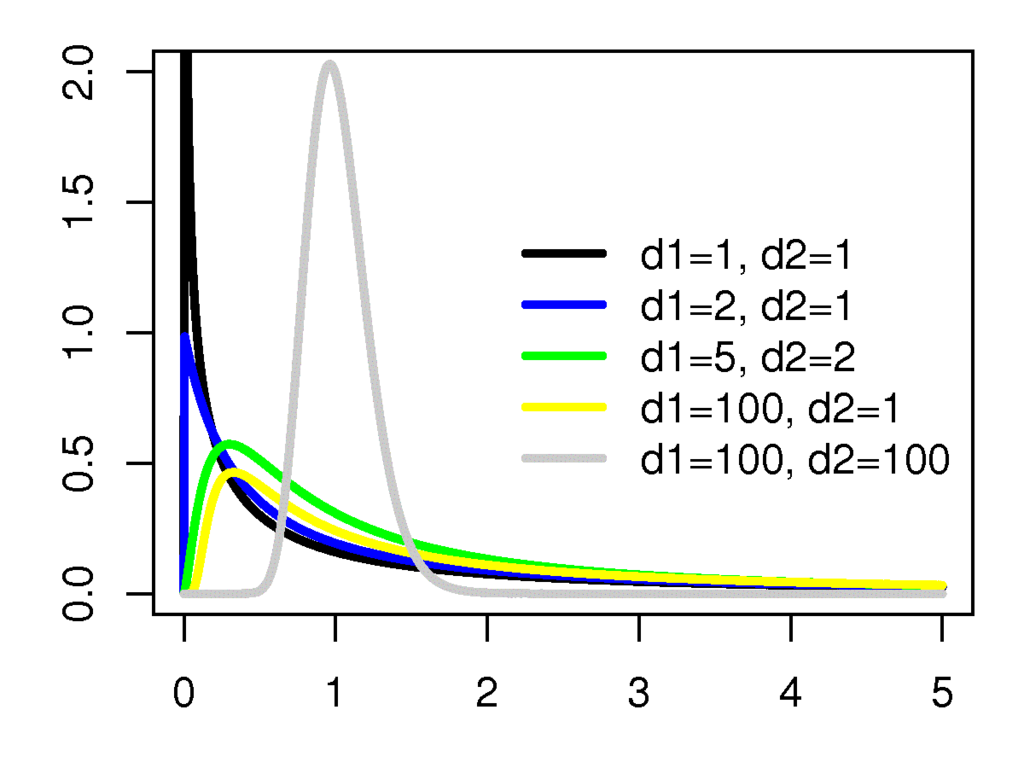
\includegraphics[scale=1.5]{imgs/f-pdf.png}
	
	\textit{PDF}
\end{center}

\begin{center}
	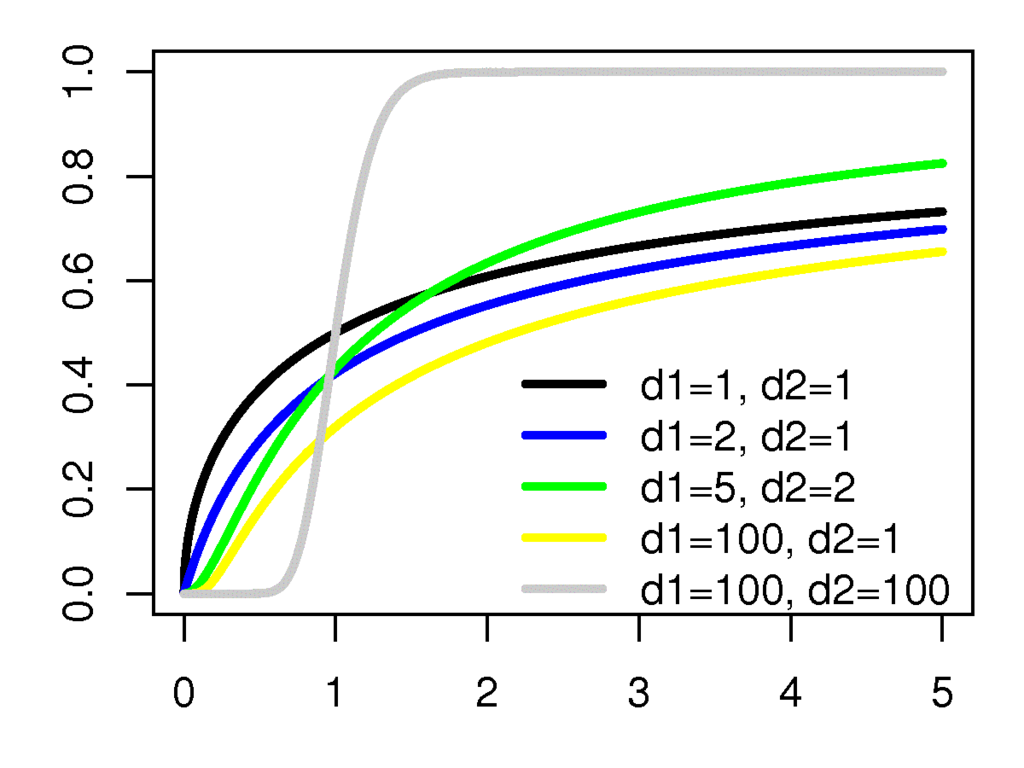
\includegraphics[scale=1.5]{imgs/f-cdf.png}
	
	\textit{CDF}
\end{center}

\section{Aplicaciones en la vida real}
La aplicación fundamental de la distribución F es la comparación de varianzas, es decir, el contraste de hipótesis referentes a varianzas de poblaciones normales e independientes, y a la comparación de medias de varias poblaciones, que constituye precisamente el “análisis de la varianza”.
\chapter{Distribución $ \Gamma $ (Gamma) }
Este modelo es una generalización del modelo \textit{exponencial}.

\section{Descripción}
Se utiliza para modelar  variables que describen el tiempo hasta que se produce p veces un determinado suceso. \cite{wiki:3}

\section{PDF}
\begin{center}
	$ f(x) = \frac{\beta^\alpha}{\Gamma(\alpha)} x^{\alpha - 1} e^{\beta x}$
\end{center}

\subsection{Parámetros}
Los parámetros observables son:

\begin{center}
	\begin{tabular} {| l | l |}
		\hline
		$\alpha$ & shape parameter\\ \hline
		$\beta$ & shape parameter\\ \hline		
	\end{tabular}
\end{center}

\section{CDF}
\begin{center}
	$ f(X < x) = \frac{1}{\Gamma(\alpha)} \gamma{\alpha, \beta x}$
\end{center}

\section{MGF}
\begin{center}
	$ m = (1 - \frac{t}{\beta})^{\alpha}$
\end{center}
\section{Media y Varianza}
\subsection{Media}
\begin{center}
	$E(x) = \frac{\alpha}{\beta}$
\end{center}

\subsection{Varianza}
\begin{center}
	$Var(x) = \frac{\alpha}{\beta^2}$
\end{center}

\section{Gráficas}

\begin{center}
	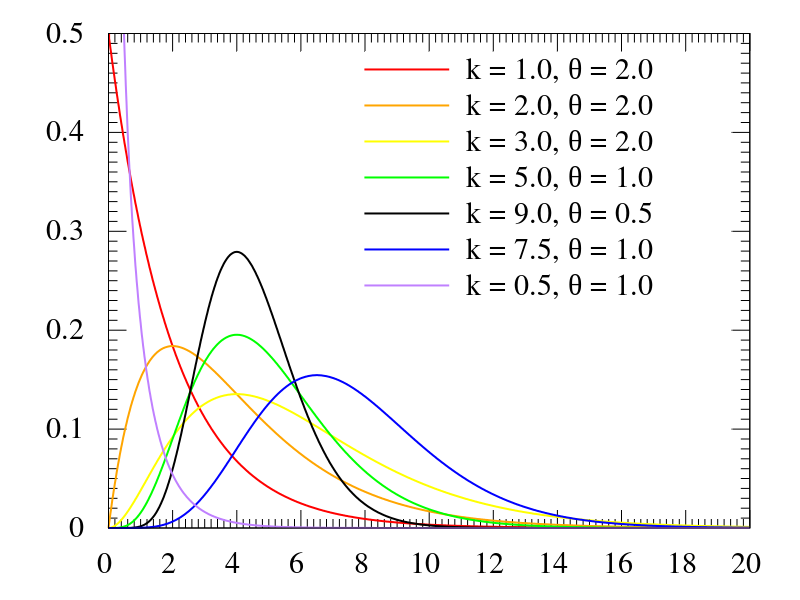
\includegraphics[scale=0.5]{imgs/gamma-pdf.png}
	
	\textit{PDF}
\end{center}

\begin{center}
	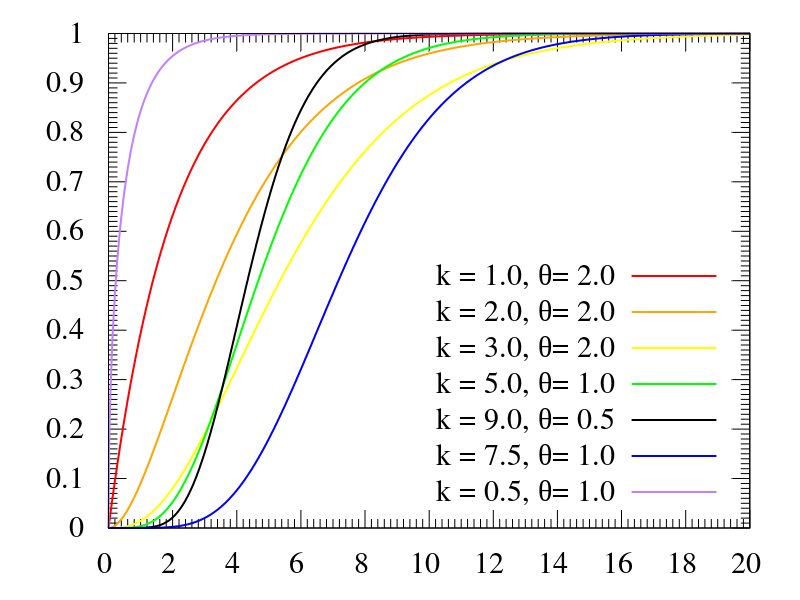
\includegraphics[scale=0.5]{imgs/gamma-cdf.png}
	
	\textit{CDF}
\end{center}

\section{Aplicaciones en la vida real}
Comunmente es usado para determinar el tiempo necesario para observar eventos en un intervalo definido.

Por ejemplo: Edad para contraer matrimonio, tiempo de fallas de sistemas...

\chapter{Distribución $ \chi^2 $}
En estadística, la distribución de Pearson, llamada también ji cuadrada(o) o chi cuadrado(a) ($ \chi^2 $), es una distribución de probabilidad continua con un parámetro  k que representa los grados de libertad de la variable aleatoria

\section{Descripción}
En realidad la distribución ji-cuadrada es la distribución muestral de $s^2$. O sea que si se extraen todas las muestras posibles de una población normal y a cada muestra se le calcula su varianza, se obtendrá la distribución muestral de varianzas. \cite{wiki:4}

\section{PDF}
\begin{center}
	$\frac {(1/2)^{k/2}}{\Gamma (k/2)} x^{k/2-1}e^{-x/2}$
\end{center}

\subsection{Parámetros}
		
\section{CDF}
\begin{center}
	$\frac {\gamma (k/2,x/2)}{\Gamma (k/2)}$
\end{center}

\section{MGF}
\begin{center}
	$(1-2\,t)^{-k/2}$
\end{center}

\section{Media y Varianza}
\subsection{Media}
\begin{center}
	$E(X) = k$
\end{center}

\subsection{Varianza}
\begin{center}
	$var(X) = 2k$
\end{center}

\section{Gráficas}
\begin{center}
	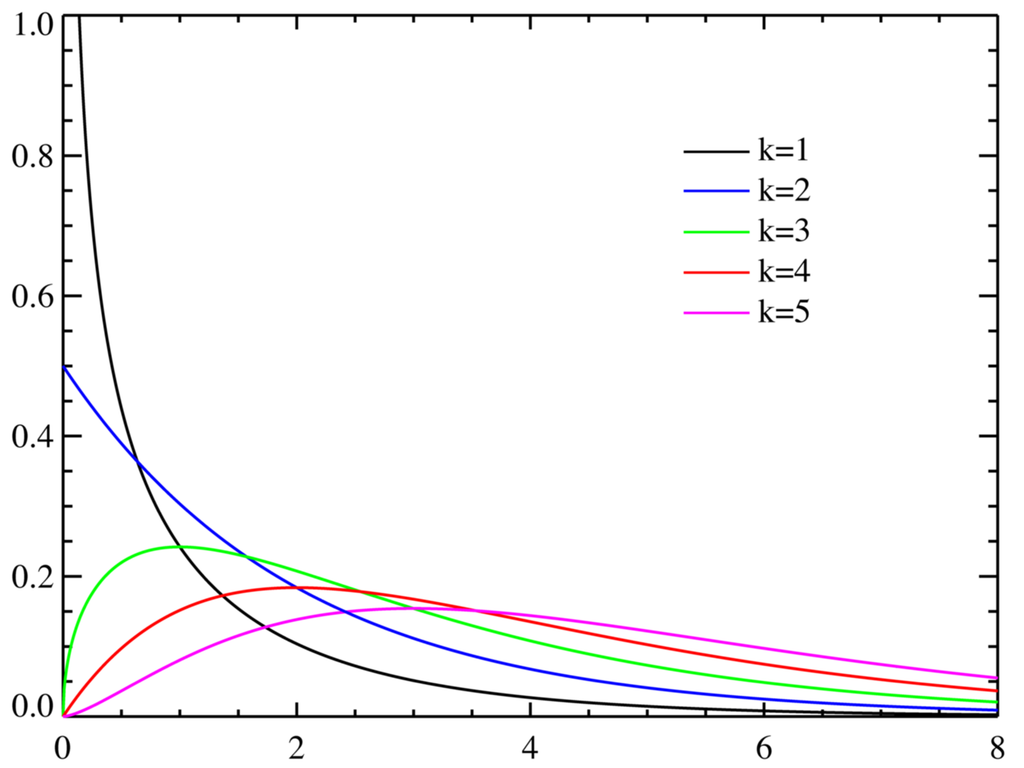
\includegraphics[scale=0.5]{imgs/chi-pdf.png}
	
	\textit{PDF}
\end{center}

\begin{center}
	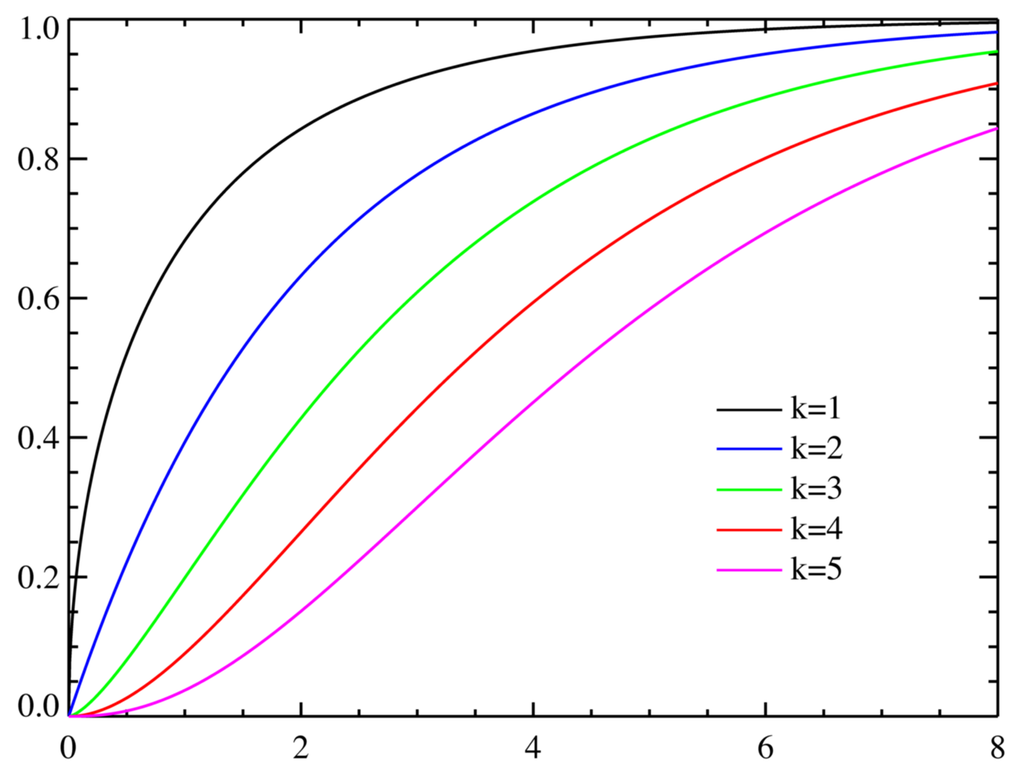
\includegraphics[scale=0.5]{imgs/chi-cdf.png}
	
	\textit{CDF}
	\end{center}

\section{Aplicaciones en la vida real}
Utilizada como prueba de independencia y como prueba de bondad de ajuste y en la estimación de varianzas. Pero también está involucrada en el problema de estimar la media de una población normalmente distribuida y en el problema de estimar la pendiente de una recta de regresión lineal, a través de su papel en la distribución t de Student.
\chapter{Distribución de Laplace}

En estadística y en teoría de la probabilidad la distribución de Laplace es una densidad de probabilidad continua, llamada así en honor a Pierre-Simon Laplace. Es también conocida como distribución doble exponencial puesto que puede ser considerada como la relación las densidades de dos distribuciones exponenciales adyacentes. \cite{wiki:5}

\section{Descripción}

Se utiliza la distribución de Laplace cuando la distribución de los datos tenga un pico más alto que una distribución normal.Por ejemplo, la distribución de Laplace se utiliza para modelar en biología, finanzas y economía.

\section{PDF}
\begin{center}
	$\frac {1}{2,b} \exp(-\frac {|x-\mu|}{b})$
\end{center}
\subsection{Parámetros}
Los parámetros observables son:

\begin{center}
	\begin{tabular} {| l | l |}
		\hline
		$\mu$ & Parámetro de localización \\ \hline
		b & Parámetro de escala\\ \hline
	\end{tabular}
\end{center}

\section{CDF}
\begin{center}
	$\frac {1}{2} \exp(\frac {x-\mu}{b})$
\end{center}

\section{MGF}
\begin{center}
	$\frac{\exp(\mu \,t)}{1-b^{2}\,t^{2}}$
\end{center}

\section{Media y Varianza}
\subsection{Media}
\begin{center}
	$\mu$
\end{center}

\subsection{Varianza}
\begin{center}
	$2b^2$
\end{center}
	
\section{Gráficas}
\begin{center}
	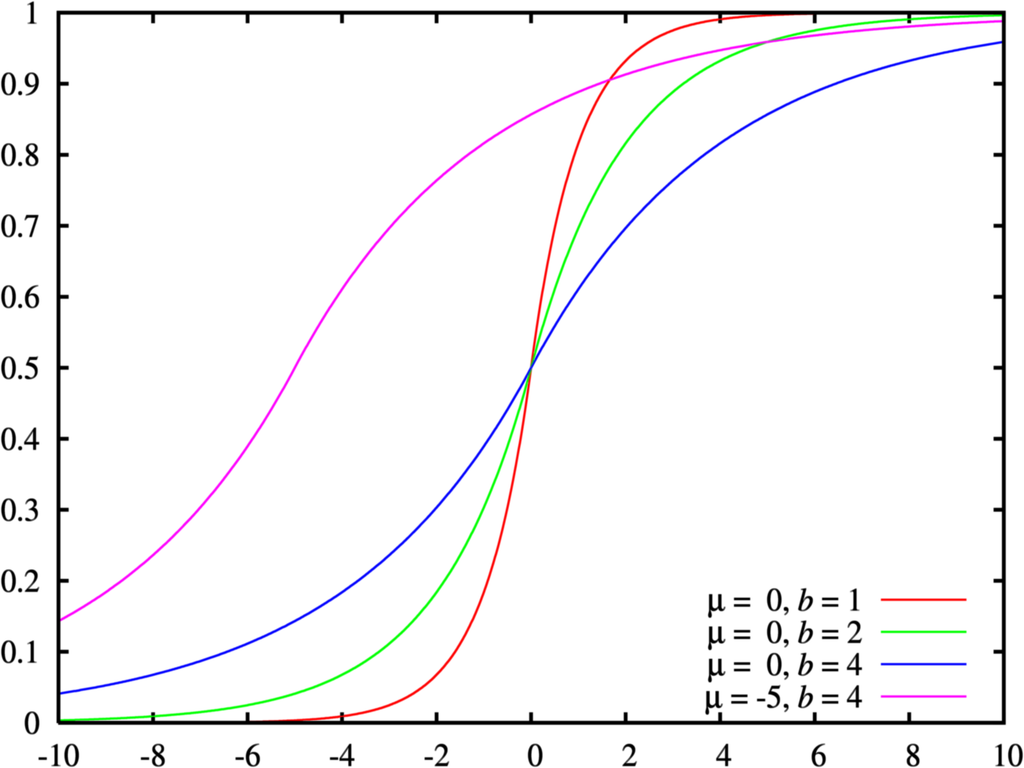
\includegraphics[scale=0.3]{imgs/laplace-cdf.png}
	
	\textit{CDF}
\end{center}

\begin{center}
	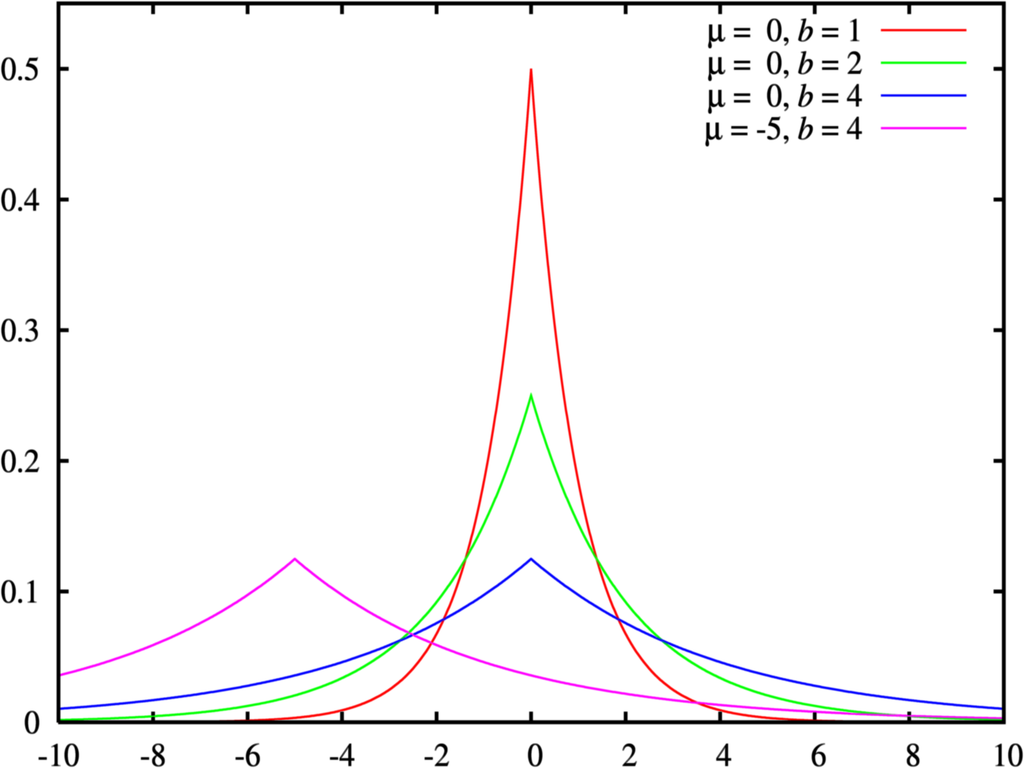
\includegraphics[scale=0.3]{imgs/laplace-pdf.png}
	
	\textit{PDF}
\end{center}
	
\section{Aplicaciones en la vida real}
La distribución laplaciana se ha utilizado en el reconocimiento de voz y en la compresión de imágenes JPEG.
\chapter{Conclusiones}

Sin duda alguna, la estadística es una campo de la ciencia que tiene mucha aplicación en nuestra vida.

Tengo la oportunidad de trabajar en una empresa donde se trabaja Inteligencia Artificial, y la estadística está intrínseca en el qué hacer diario.

Creo que junto a la Investigación de Operaciones, este ha sido un curso de los que puedes ver aplicados día a día en nuestra vida.


%now enable appendix numbering format and include any appendices
%\appendix
%\include{appendix1}

%next line adds the Bibliography to the contents page
\addcontentsline{toc}{chapter}{Bibliography}
%uncomment next line to change bibliography name to references
%\renewcommand{\bibname}{References}
\bibliography{refs}        %use a bibtex bibliography file refs.bib
\bibliographystyle{plain}  %use the plain bibliography style

\end{document}

